\chapter{Development of a new polarizability functional}\label{chap:polarizability}

The work presented in the last chapter is motivated by a development of a unified and more general vdW method based on the MBD framework (Section~\ref{sec:mbd}).
As shown in Chapter~\ref{chap:pi-pi} and elsewhere \citep{HermannCR17}, many-body effects can play a profound role in vdW interactions, and the MBD approach is thus an appropriate starting point for a general and accurate vdW model.
But the parametrization of the harmonic oscillators based on the free-atom reference values and Hirshfeld-volume scaling used in the MBD method has several disadvantages compared to the local polarizability models of nonlocal density functionals (Section~\ref{sec:vdwdf}).
First, the Hirshfeld-volume model is based on the assumption that the electron density of atoms in molecules and materials is not qualitatively different from isolated atoms, but only contracted to a certain degree by the environment.
This is largely the case in systems without strong charge transfer between atoms, but fails considerably in ions, where the added or removed electrons change the electron density significantly, as well as in metals, where the electrons in the conducting bands are completely delocalized from atoms.
Second, the Hirshfeld-volume parametrization provides only two of the three parameters that specify a harmonic oscillator (for instance $(m,q,\omega)$ or $(\alpha(0),C_6,m)$).
Whereas these two parameters, $\alpha(0)$ and $\omega$ (or equivalently $C_6$), fix the asymptotic long-range interaction, they do not give sufficient information to fix the width of the oscillators.
This limitation is avoided either by using the (ambiguous) atomic vdW radii to range-separate the MBD Hamiltonian, or with a semi-classical expression for the oscillator width in terms of the dipole polarizability, which is used in the dipole-screening equation.
Besides introducing empirical elements into the model, neither of these approaches can be easily generalized to describe anisotropy in the range separation.
Third, the Hirshfeld-volume scheme is inherently tied to atomic partitioning.
If, say, one wanted to place additional harmonic oscillators on the centers of covalent bonds, the Hirshfeld partitioning could not support such a model.
None of these issues are shared by local polarizability functionals.
They have no inherent bias towards neutral atoms, the third oscillator parameter can be obtained from the spatial distribution of the polarizability as quadrupole polarizability (Section~\ref{sec:quadrupole}), and any partitioning of space can be directly used to partition the polarizability and formulate a MBD-like fragment-based method.
This chapter investigates the use of polarizability functionals in formulation of a MBD-based vdW method.

In the next section, we analyze how the local polarizability functional yields quadrupole polarizabilities of the interacting fragments, and how these can be used to naturally define the range separation in the MBD approach.
The following section then investigates the accuracy of existing polarizability functionals across the periodic table, analyzes the failures, and presents a new functional that is more accurate.
The third section deals with the connection between the polarizability functionals and the volume-scaling approach, by comparing the scaling power laws predicted by the functionals to reference benchmark values.
Finally, we present an outlook on how to incorporate a local polarizability functional into a complete MBD-based vdW method.

\section{Quadrupole polarizability from polarizability functional}\label{sec:quadrupole}

The quadrupole--quadrupole polarizability of an object (isolated atom, any fragment of a molecule, a molecule) is an operator that relates the electric field on the object generated by a distant electric quadrupole to the induced quadrupole moment on the object.
Equivalently, it can also be defined as a quadrupole response of the object to a gradient of the electric field.
For spherically symmetric objects, such as isolated atoms, the quadrupole--quadrupole polarizability is the lowest nonzero multipole moment of the polarizability after the lowest dipole--dipole moment.
Here, we derive the quadrupole--quadrupole polarizability of an object defined by a spatial distribution of the dipole polarizability, which is the model represented by any local polarizability functional.

Consider an object with a local polarizability density, $\boldsymbol\alpha(\mathbf r)$, under an influence of an external electric field of the form $\mathbf E(\mathbf r)=\mathbf E'\mathbf r$, $\mathbf E'$ being the (constant) spatial derivative of the field, $\nabla_i E_j(\mathbf r)=E'_{ji}$.
The field will induce dipole polarization, $\mathbf P=\boldsymbol\alpha\mathbf E'\mathbf r$, which can be represented by a superposition of two constant charge densities of the opposite sign, $\pm q$, shifted microscopically by $\pm\mathbf P(\mathbf r)/2q$ at each point.
The resulting induced quadrupole moment, $\mathbf Q$, can then be calculated as
\begin{equation}
\begin{aligned}
Q_{ij}&=\int\mathrm d\mathbf r\,n(\mathbf r)\tfrac12(3r_i r_j-r^2\delta_{ij}) \\
&=\sum_\pm\,\pm q\int\mathrm d\mathbf r\,\tfrac12\big[3\big(r_i\pm\tfrac1{2q}P_i(\mathbf r)\big)\big(r_j\pm\tfrac1{2q}P_j(\mathbf r)\big)-\big|\mathbf r\pm\tfrac1{2q}\mathbf P(\mathbf r)\big|^2\delta_{ij}\big] \\
&=\sum_\pm\,\pm q\int\mathrm d\mathbf r\,\tfrac12\big[3\big(r_i r_j\pm\tfrac1{2q}(r_i P_j(\mathbf r)+r_j P_i(\mathbf r)\!)\big)-\big(r^2\pm\tfrac1q\mathbf r\cdot\mathbf P(\mathbf r)\!\big)\delta_{ij}]\\
&=\int\mathrm d\mathbf r\,\tfrac12\big[3\big(r_i P_j(\mathbf r)+r_j P_i(\mathbf r)\!\big)-2{\textstyle\sum_m}r_m P_m(\mathbf r)\delta_{ij}] \\
&=\sum_{kl}\int\mathrm d\mathbf r\,\tfrac12\big[3\big(r_i r_l\alpha_{jk}(\mathbf r)+r_j r_l\alpha_{ik}(\mathbf r)\!\big)-2{\textstyle\sum_m}r_m r_l\alpha_{mk}(\mathbf r)\delta_{ij}]E'_{kl} \\
&=\sum_{kl}C_{ijkl}\delta_{ij}E'_{kl}
\end{aligned}
\end{equation}
Here, $C_{ijkl}$ is the quadrupole--quadrupole polarizability of the object in Cartesian coordinates.

All existing polarizability functionals as well as the new ones introduced in this chapter are isotropic, $\alpha_{ij}(\mathbf r)=\alpha(\mathbf r)\delta_{ij}$, so that
\begin{equation}
C_{ijkl}=\int\mathrm d\mathbf r\,\tfrac12\big[3\big(r_i r_l\delta_{jk}+r_j r_l\delta_{ik}\!\big)-2{\textstyle\sum_m}r_m r_l\delta_{mk}\delta_{ij}\big]\alpha(\mathbf r)
\end{equation}
As a result, the quadrupole--quadrupole polarizability can be anisotropic even with an isotropic polarizability functional, as long as the density of the object is anisotropic.
This is in contrast to the coarse-grained dipole--dipole polarizabilities, which are always isotropic when calculated from an isotropic polarizability functional, regardless of the spatial distribution of the polarizability.

For isotropic objects (such as isolated atoms), however, both dipole--dipole and quadrupole--quadrupole polarizabilities are isotropic.
This result can be obtained by setting $r_i r_j=\delta_{ij}r^2/3$ in the expression above, which is valid if the integral is over the whole space and the integrand is radially symmetric,
\begin{equation}
C_{ijkl}=\tfrac12(\delta_{il}\delta_{jk}+\delta_{jl}\delta_{ik}-\tfrac23\delta_{kl}\delta_{ij})\int\mathrm d\mathbf r\,\alpha(\mathbf r)r^2
\end{equation}
Here, $\mathbf C$ is an isotropic traceless 4th-order tensor as expected.
In the solid-harmonic basis (Section~\ref{sec:coarse-graining}), the corresponding quadrupole polarizability is expressed as
\begin{equation}
  \alpha_{22,mm'}=\delta_{mm'}\alpha_2=\delta_{mm'}\int\mathrm d\mathbf r\,\alpha(\mathbf r)r^2
  \label{eq:iso-quadrupole}
\end{equation}

\begin{figure}[t]
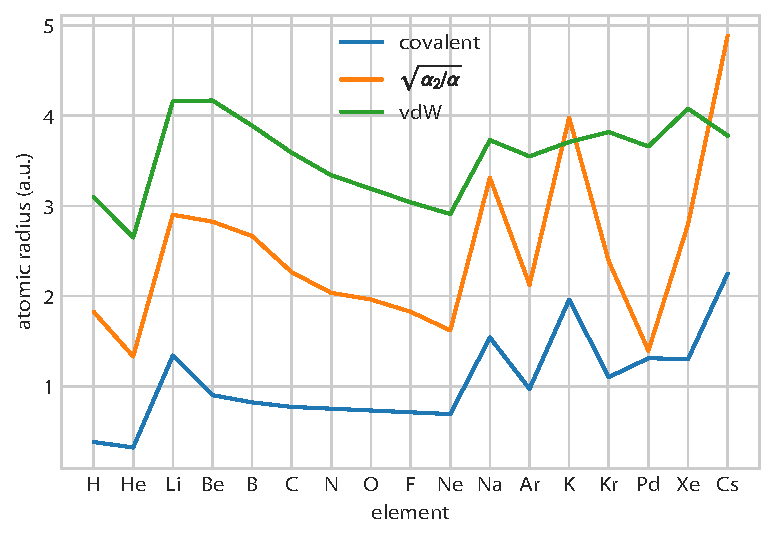
\includegraphics{media/pol-radii.pdf}
\caption{\textbf{Comparison of different definitions of atomic radii.}
Covalent radii are taken from \citep{CorderoDT08}, vdW radii from \citep{TkatchenkoPRL09,BondiJPC64}.
The atomic radius defined from the ratio of the quadrupole and dipole polarizability (yellow) is derived in~\eqref{eq:pol-radius}.
}\label{fig:pol-radii}
\end{figure}

The formula above provides a particularly simple interpretation of the quadrupole polarizability as a second radial moment of the local polarizability distribution.
In this regard, it encodes information about the spatial distribution of the polarizability density, and hence can naturally define the width of the oscillators in the MBD model.
In particular, the Gaussian width, $\sigma^2$, (see eq.~\ref{eq:mayer}) of the particle density of a quantum harmonic oscillator in ground state is equal to $1/m\omega=3\alpha_2(0)/4\alpha(0)$.
By substituting~\eqref{eq:iso-quadrupole}, we get
\begin{equation}
  \sigma^2=\frac34\frac{\int\mathrm d\mathbf r\,r^2\alpha(\mathbf r,u=0)}{\int\mathrm d\mathbf r\,\alpha(\mathbf r,u=0)}
\end{equation}

Interestingly, this interpretation of the quadrupole polarizability also yields a new possible definition of atomic radii based on polarizabilities.
Assume a model of an atom as a thin spherical shell (representing the valence electrons), where all the polarization response is concentrated at distance $R_\text{pol}$.
It then follows that this radius must satisfy
\begin{equation}
  R_\text{pol}=\sqrt{\frac{\alpha_2(0)}{\alpha(0)}}
  \label{eq:pol-radius}
\end{equation}
The magnitude of this ``polarizability radius'' is between covalent and vdW radii for most atoms (Figure~\ref{fig:pol-radii}).
Like vdW radii and unlike covalent radii, the polarizability radii decrease within the second row.
Like covalent radii and unlike vdW radii, the polarizability radii of alkali atoms are substantially larger than those of the noble-gas atoms in the same period, and they grow with increasing atomic number.
For palladium, the only transition-metal element in the set, the polarizability radius is almost equal to the covalent radius.

\section{Constructing orbital-dependent polarizability functionals}\label{sec:new-functionals}

In this section, we generalize the VV polarizability functional (eq.~\ref{eq:vv-pol}) to achieve a more balanced performance across the periodic table.
This is a first necessary step if the Hirshfeld-scaling is to be replaced with a local polarizability functional without deteriorating accuracy, because the former is exact for isolated atoms by construction.
The general form of the VV functional is
\begin{equation}
  \alpha_\text{VV}[n](\mathrm iu)=\frac{n}{An+B|\boldsymbol\nabla n/n|^4+u^2}
\end{equation}
In the VV functional, $A=\frac13\times4\pi\doteq4.2$ is set such that the asymptotic interaction of two spheres of uniform electron gas is reproduced exactly.
This value of $A$ can be also derived from the Clausius--Mossotti equation by taking the dielectric function of the uniform electron gas.
But both these arguments have shortcomings.
The local polarizability functional is supposed to take into account only exchange and local correlation effects, not the fully nonlocal electron correlation.
If it was used in a many-body vdW model to describe the two uniform-gas spheres, the long-range screening would be described explicitly by the model, and should not be accounted for in the polarizability functional.
Furthermore, the asymptotic interaction between the spheres was calculated semi-classically~\cite{LucasPRB75} without considering any edge effects on the boundary of the sphere where true electron density would decay continuously outside the spherical positively-charged compensating background.
The Clausius--Mossotti relation between microscopic polarizability and macroscopic dielectric function is valid only for dielectric materials, which the uniform gas is not, and furthermore, the used Lindhard formula for the dielectric function is only approximate and for the macroscopic response equal to the classical Drude model.
In this regard, we consider the particular choice of the value of the parameter $A$ rather arbitrary.

The value of the parameter $B\doteq0.0089$ was fitted to reproduce reference $C_6$ coefficients in the VV functional.
But the following simple reformulation of the VV form gives a clear interpretation of this numerical value.
The local resonance frequency, $\omega^2=An+B|\boldsymbol\nabla n/n|^4$, is a measure of the electron delocalization---delocalized electrons are more polarizable.
Another measure of delocalization is the kinetic energy, which can be seen for example from the local expansion of the electron pair correlation function in~\eqref{eq:pair-correlation-expansion}.
Correspondingly, the VV functional can be rewritten in terms of the von Weizsäcker kinetic energy functional,
\begin{equation}
  \alpha_\text{VV}[n](\mathrm iu)=\frac{n}{An+(B'\tau_\text W/n)^2+u^2}
\end{equation}
Here, $B'=8\sqrt{B}\doteq0.75$.
The ratio $\tau_\text W/n$ in the density tail of any finite electronic system is equal to the ionization potential, while $\omega$ measures the local effective electronic gap.
The value of 0.75 corresponds for instance to the $1s\rightarrow2p$ transition in the hydrogen atom, which is the lowest-energy transition that contributes to the dipole polarizability.
In this sense, the term $An$ can be considered as an effective damping that captures the contributions of the higher-energy transitions to the polarizability.

\begin{figure}
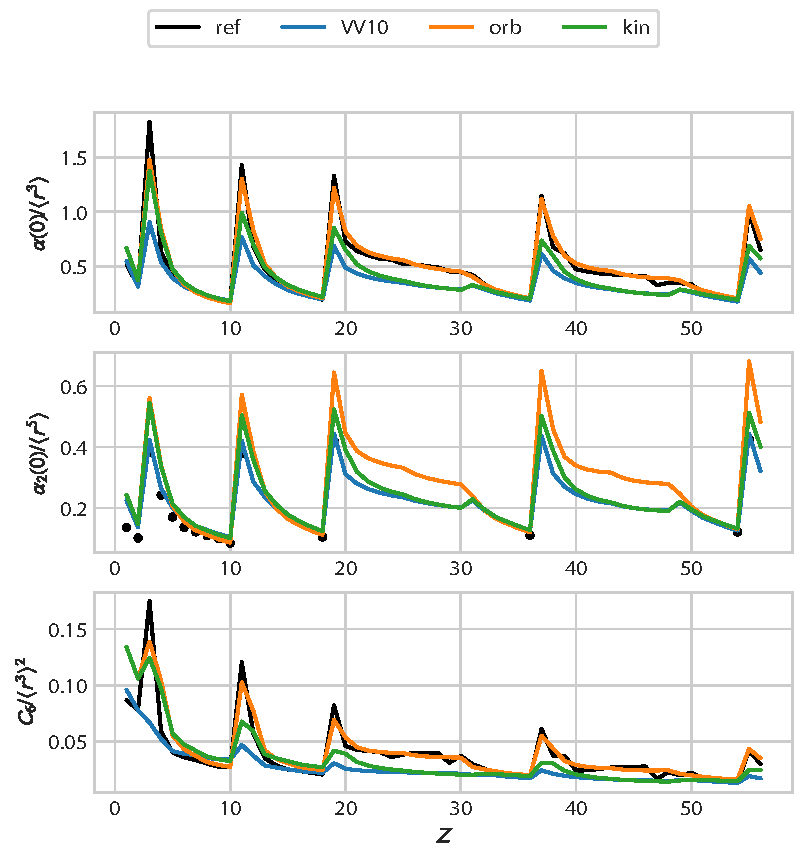
\includegraphics{media/pol-periodic-table.pdf}
\caption{\textbf{VdW parameters across periodic table predicted with polarizability functionals.}
From top to bottom, the plots are of the dipole polarizability with respect to the Hirshfeld volume ($\langle r^5\rangle$), the quadrupole polarizability with respect to $\langle r^5\rangle$, and the homonuclear $C_6$ coefficient with respect to the square of the Hirshfeld volume.
$Z$ is the atomic number.
Plotted are the reference values (black) for the dipole polarizabilities, $C_6$ coefficients \citep{GouldJCTC16}, and quadrupole polarizabilities \citep{AbdalmoneamJPBAMOP14,SchmidtPRB79,SternheimerPRA70,ReinschPRA78,SahooCPL07,KomasaPRA01}, as well as the values obtained from the VV10 polarizability functional and the functionals developed in Section~\ref{sec:new-functionals}.
}\label{fig:pol-periodic-table}
\end{figure}

\begin{figure}
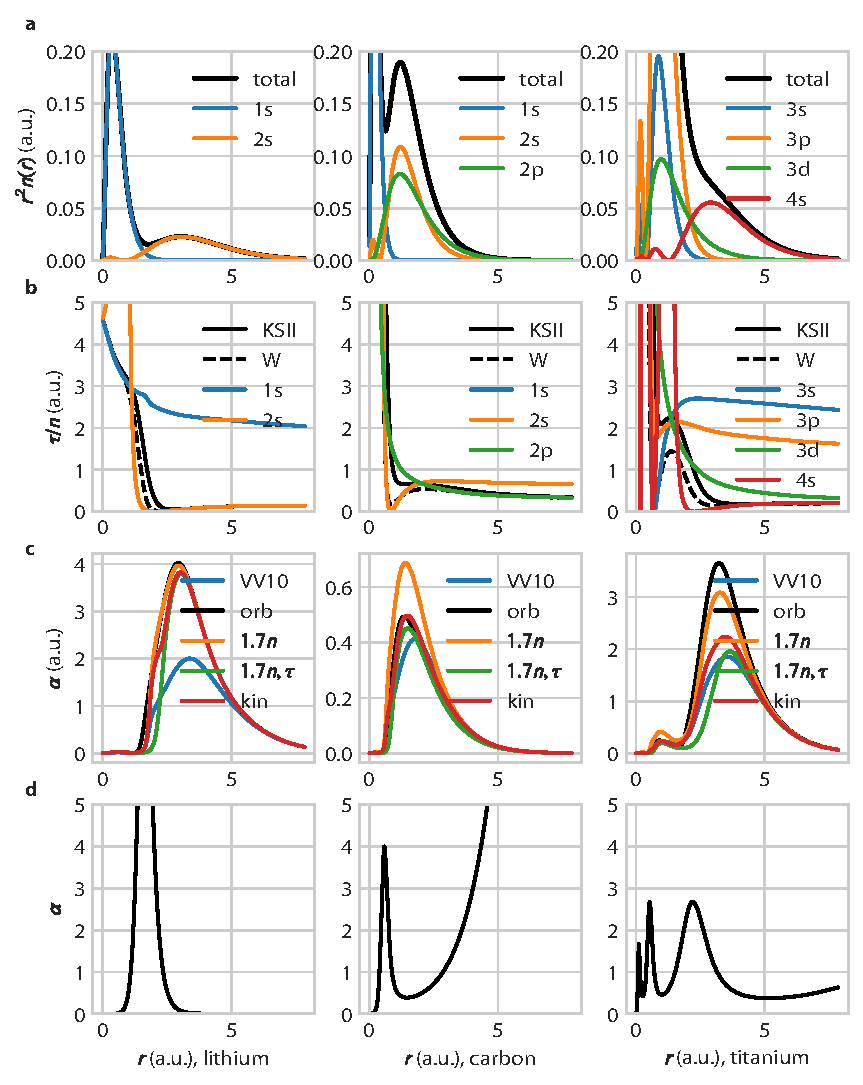
\includegraphics{media/atomic-densities.pdf}
\caption{\textbf{Polarizability functionals and isolated atoms.}
The plots show several density-based quantities in radially symmetric isolated atoms of lithium ([He]\,2s$^1$), carbon ([He]\,2s$^2$2p$^2$), and titanium ([Ar]\,3d$^2$4s$^2$) in columns from left to right.
(\textbf a) Radial plots of the total electron density (black), $r^2n(r)$, and its decomposition into individual electron orbitals.
nd 
(\textbf b) The KS kinetic-energy density of the second kind (black, eq.~\ref{eq:kinetic}), its decomposition into electron orbitals, and the von Weizsäcker kinetic-energy functional (black, dashed, eq.~\ref{eq:von-w}).
(\textbf c) Local polarizability density from the VV functional as well as new functionals developed in Section~\ref{sec:new-functionals}.
(\textbf d) The electron-localization parameter $\alpha$ (eq.~\ref{eq:scan-alpha}).
}\label{fig:atomic-densities}
\end{figure}

To evaluate the performance of the VV polarizability functional for atoms across the periodic table, we have calculated the dipole and quadrupole polarizabilities and $C_6$ coefficients for all atoms up to barium (Figure~\ref{fig:pol-periodic-table}).
We used KS-DFT with the PBE functional and a radial atomic solver to calculate the electronic structure.
In general, the VV functional gives reasonable static polarizabilities and $C_6$ coefficients for $p$-block elements, but underestimates them both for $d$-block metals and even more for $s$-block metals.
Surprisingly, static quadrupole polarizabilities are predicted quite accurately even for $s$-block metals.
In terms of a local polarizability model, this can be interpreted such that the response is estimated correctly in the density tails, which dominate the radial contribution to the quadrupole polarizability (due to the $r^2$ factor in~\eqref{eq:iso-quadrupole}), but severely underestimated closer to the nucleus for the $s$- and $d$-metals.
To better understand this failure, we have analyzed the individual orbital contributions to the electron density and the different models of the local kinetic energy density (Figure~\ref{fig:atomic-densities}).
Comparison of the lithium ($s$), carbon ($p$), and titanium ($d$) atoms suggests that the differences in the performance between the three blocks of the periodic table may stem from the fact that although the valence electrons are responsible for most of the electronic response (unlike the XC energy, which is dominated by the inner shells), the electron density of the inner electronic shells shields the valence density.
A functional that only ``sees'' the total density cannot recognize between the inner and valence shells, which then leads to the underestimation of the polarizability.
This explanation is also in line with the accurate prediction of the quadrupole polarizabilities, which are mostly determined by the regions of the electron density beyond the overlap of the valence and inner shells.

To test this hypothesis, we formulate a generalization of the VV functional that applies a VV-like form to the individual KS orbitals,
\begin{equation}
  \alpha_\text{orb}(\mathbf r,\mathrm iu)=\sum_i\frac{f_i|\phi_i(\mathbf r)|^2}{An(\mathbf r)+(B'|\boldsymbol\nabla\phi_i(\mathbf r)|^2/2|\phi_i(\mathbf r)|^2)^2+u^2}
\end{equation}
Here, $f_i$ is the occupation number of the $i$-th orbital, $|\phi_i(\mathbf r)|^2$ is its normalized electron density, and $|\boldsymbol\nabla\phi_i(\mathbf r)|^2/2$ its contribution to the KS kinetic energy density of the first kind, $\tau_\text{I}$ (eq.~\ref{eq:kinetic}).
To retain the good performance of the VV functional for quadrupole polarizabilities, we keep the parameter $B'$ fixed at the VV value, and optimize $A=1.7$ by minimizing the mean absolute relative error in the polarizabilities.
Figure~\ref{fig:pol-periodic-table} shows that the new functional, denoted ``orb'', improves upon the VV functional for the $s$- and $d$-block elements, while having the same accuracy for the $p$-block species, both in terms of the dipole polarizabilities and $C_6$ coefficients.
Compared to the VV functional, the quadrupole polarizabilities are somewhat overestimated for the $s$-block elements, and there are no available reference data for the $d$-block elements.

The improved performance of the orbital-dependent formulation is promising, but has a theoretical drawback---namely, it is not invariant with respect to orbital rotation.
This introduces certain arbitrariness in the model, and makes it computationally more demanding for evaluation in atom-centered basis sets, because the functional cannot be formulated in terms of the density matrix.
Figure~\ref{fig:atomic-densities}d shows that the inter-shell regions are well distinguished by the density parameter $\alpha$ (eq.~\eqref{eq:scan-alpha}).
As a result, the orbital dependence can be simulated by interpolating between the KS kinetic energy density and the von Weizsäcker functional, which is accurate in the intra-shell regions,
\begin{equation}
  \alpha_\text{kin}[n](\mathrm iu)=\frac{n}{An+f(\alpha[n])(B'\tau_\text W/n)^2+(1-f(\alpha[n]))(B'\tau_\text{KS}^\text{II}/n)^2+u^2}
\end{equation}
We choose an arbitrary sigmoid function for the interpolation, $f(\alpha)=(1+(\alpha-1)/\sqrt{1+(\alpha-1)^2})/2$, with the switching point at $\alpha=1$, the value that $\alpha$ has in the uniform electron gas.
Figure~\ref{fig:pol-periodic-table} shows that this formulation is a promising improvement over the VV functional for the lighter elements, but the difference between the two functionals becomes small with growing $Z$.

\section{Volume-scaling of polarizabilities with polarizability functionals}

\begin{figure}
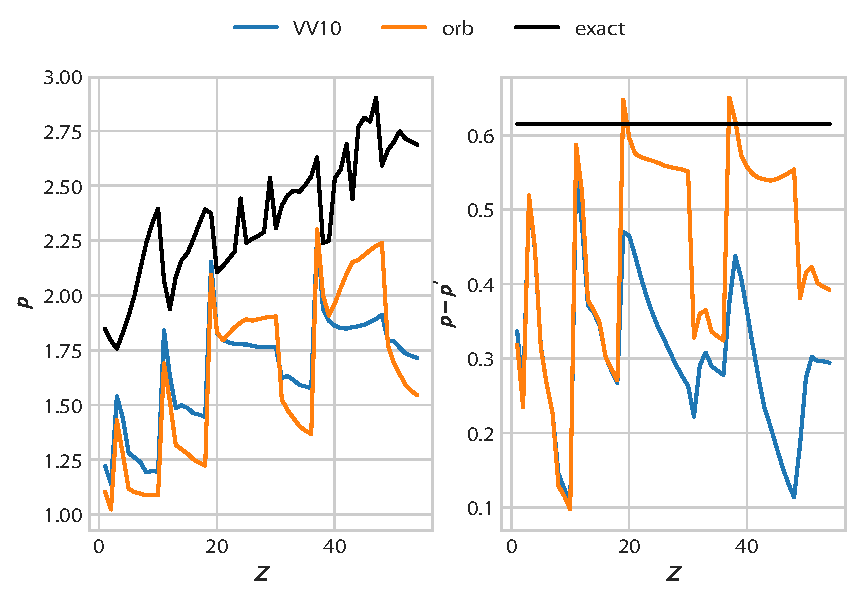
\includegraphics{media/pol-scaling.pdf}
\caption{\textbf{Scaling of atomic polarizabilities and $C_6$ coefficients with Hirshfeld volumes.}
$Z$ is the atomic number.
The power-law scaling is defined as $\alpha(0)/\alpha_\text{free}(0)=(V/V_\text{free})^{p'}$ and $C_6/C_{6,\text{free}}=(V/V_\text{free})^{p}$, with the contracted atoms defined by confining with an external potential of the form $r^2/r_\text{c}^3$.
The reference values for $p$ and $p'$ are taken from \citep{GouldJCP16}.
The reference constant difference $p-p'\approx0.615$ is accurate to within $0.1$ for most elements.
}\label{fig:pol-scaling}
\end{figure}

The polarizability functional should serve as a replacement for the TS volume-scaling approach in the unified MBD model.
The TS model assumes (Section~\ref{sec:pairwise}) that the polarizability of an atom scales linearly with its Hirshfeld volume ($p=1$), and the $C_6$ coefficient with the square of the volume ($p'=2$).
On the other hand, \citet{GouldJCP16} calculated accurate polarizabilities and $C_6$ coefficients of confined atoms with TD-DFT and found that $p$ and $p'$ depend substantially on the atomic number, and range from 1.75 to 2.75 and from 1.15 to 2.1, respectively.
We have calculated the scaling coefficients $p$ and $p'$ as predicted by the polarizability functionals VV and ``orb'' by evaluating them on the electron densities of the confined atoms (Figure~\ref{fig:pol-scaling}).
In contrast to the polarizabilities and $C_6$ coefficients, the volume-scaling behavior is represented rather poorly by the polarizability functionals both qualitatively and quantitatively.
The scaling coefficients are underestimated, and the trends within each period of the periodic table are reversed.
No significant difference is observed between the VV and ``orb'' functionals.

\begin{figure}
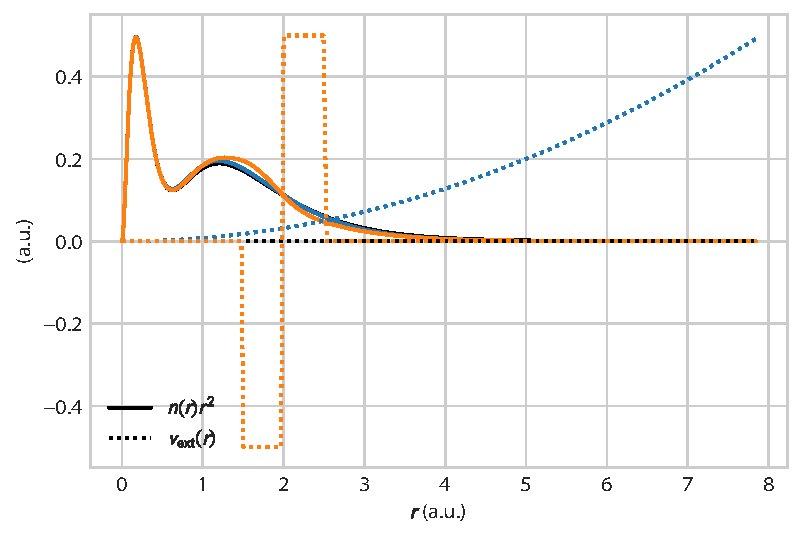
\includegraphics{media/scaling-c.pdf}
\caption{\textbf{The effect of different confinement potentials on the carbon atom.}
The radial quadratic potential (blue) and the radial localized potential at distance corresponding to the C--H distance in methane (yellow) yield the same change in the Hirshfeld volume.
}\label{fig:scaling-c}
\end{figure}

To understand better this failure, we investigated the dependence of the scaling behavior on the confining potential.
\citeauthor{GouldJCP16} tested polynomial potentials of the form $r^n/r_\text{c}^{n+1}$, with $n=2,3,4$, and found only negligible dependence on $n$.
But these three potentials are qualitatively similar, and quite different from the confinement that acts on atoms in molecules.
Figure~\ref{fig:scaling-c} compares the effect on the carbon atom of the quadratic confining potential ($n=2$) and a localized step potential at a distance corresponding to the C--H distance in methane.
Although the effect on the Hirshfeld volume is the same in both cases (reduction by 20\%, c.f. 30\% in methane), the latter has a much stronger effect.
This is caused by the strong sensitivity of the Hirshfeld volume on the density-tail behavior due to the $r^3$ factor.
Likewise, the two potentials differ in their effect on the polarizability as predicted by the polarizability functionals.
Whereas the quadratic potential yields $p'=1.0$ (reference value of $p'=1.4$), the localized potential yields $p'=1.4$ (no reference available).
The same values are obtained both with the VV and ``orb'' polarizability functional.
Given the lack of available reference volume-scaling data for other than the polynomial confining potentials, these results have two potential interpretations.
Either the true volume-scaling behavior is indeed independent of the confining potential shape, and the difference in the scaling coefficients predicted by the polarizability functionals is artificial.
This would mean that the functionals perform better for more realistic confinements.
The other interpretation would be that the volume-scaling behavior depends significantly on the potential shape, in which case the reference results from the polynomial potentials do not bear much relevance to the confinement of atoms in molecules.
In either case, the large deviations of the polarizability functionals from the reference values in Figure~\ref{fig:pol-scaling} do not necessarily have implications for the accuracy of the functionals in realistic molecules and materials.

\section{Outlook on future development}

In this final section, we outline the path towards a complete MBD-based vdW model that uses the polarizability functional developed above.
The goal of such a method is to unify the accuracy of MBD with the electronic-structure universality of nonlocal vdW functionals (such as VV10).

\begin{description}
\item[Partitioning] The first step in formulating a coarse-grained model is the choice of partitioning of the space into fragments.
In the approach based on scaling free-atom values with Hirshfeld-volume ratios (the TS model), the total polarizability (even before any screening) depends on the choice of the partitioning, which makes the choice particularly important.
This is the reason why the TS method based on iterative Hirshfeld partitioning gives significantly better results for ionic system than regular Hirshfeld partitioning.
In contrast, the total polarizability of a system described by a local polarizability functional is simply an integral over the whole space, and is independent of a particular partitioning.
The choice should therefore play a less important role, and any atomic partitioning should be sufficient.
\item[Free-atom reference data] One of the core advantages of the TS method that makes it accurate is the use of reference data for free atoms.
The orbital-dependent formulation of the VV functional developed above improves its performance across the periodic table, but still is not exact.
A straightforward correction that makes the model exact for free atoms is to scale the coarse-grained polarizabilities of atoms in a molecule with the ratio of the exact and approximate polarizability of free atoms,
\begin{equation}
  \alpha_i(\mathrm iu)=\frac{\alpha_{i,\text{free,ref}}(0)}{\alpha_{i,\text{free},\alpha[n]}(0)}\int\mathrm d\mathbf r\,w_i(\mathbf r)\alpha[n](\mathbf r,\mathrm iu)
\end{equation}
\item[Polarizability screening] The use of the density gradient in GGA functionals and of the kinetic-energy density in meta-GGA functionals makes them in general longer-ranged than the LDA, which uses only the density (Chapter~\ref{chap:xc-functionals}), because the density derivatives encode more detailed information about the electronic structure.
Along the same lines, the local polarizability functionals, which use semilocal density information, can be expected to capture larger portion of the effect of neighboring atoms on the polarizability than the Hirshfeld-volume scaling that uses only the electron density.
We expect that this may render the short-range polarizability screening unnecessary.
\item[Range separation] As discussed in Section~\ref{sec:quadrupole}, the quadrupole polarizabilities that can be calculated from a local polarizability functional provide a natural measure of the width of the fragments represented by harmonic oscillators.
This enables replacing the range-separation based on vdW radii with a scheme that is independent of explicit free-atom reference, which has two advantages.
First, it enables the potential use of finer partitioning that is only partially based on atoms.
For instance, one could consider placing a fragment on each covalent bond in the system.
This would make the coarse-graining finer and would limit the errors associated with neglecting higher multipole moments.
Second, the quadrupole polarizabilities calculated even from an isotropic polarizability functional are in general anisotropic, and thus naturally lead to anisotropic range separation.
This should prove especially useful for hybrid interfaces, where the electron density on a metallic surface is strongly delocalized in the directions parallel to the surface, but localized in the perpendicular direction.
\end{description}
